\chapter{Laboratorio 1: \\Power Estimation: probabilistic techniques}
\section{Probability and Activity Calculation: Simple Logic Gates}
Durante la prima parte dell'esercitazione è stata calcolata la probabilità di avere '1' logico in uscita di alcuni gate elementari, con la relativa Switching Activity.
\begin{figure}[!htb]
	\centering
	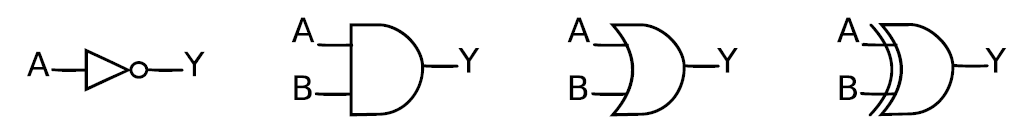
\includegraphics[scale=0.8]{immagini/gate}
	\caption{\textit{Probabilità e Switching Activity stimati manualmente}}
	\label{fig1_1}
\end{figure} \\
La probabilità di '1' logico è stata stimata semplicemente andando a valutare il rapporto fra il numero di possibili combinazioni con '1' logico diviso il numero di combinazioni totali. Invece per il calcolo della Switching Activity è stata utilizzata la formula vista a lezione:
\begin{center}
	$ A=P_{1}P_{0}+P_{1}P_{0}=2P_{1}(1-P_{1}) $
\end{center}
$\alpha$
Dove $P_{1}$ e $P_{0}$ sono le probabilità di avere '1' e '0' logici in uscita dalla mia porta. \\
In seguito, tramite il programma \textit{ModelSim} è stato analizzato il numero di toogle delle varie porte utilizzando un testbench sviluppato appositamente dai docenti. Si è andato a variare il numero di colpi di clock, come richiesto dalla traccia ed in seguito si sono comparati i valori ottenuti dalla simulazione con ciò che si era calcolato manualmente.\\
Tramite appositi comandi di Modelsim (\textbf{-power report}), sono stati stilati dei report relativi ad una stima delle commutazioni delle varie porte, della quale se ne riporta un esempio in Figura \ref{fig1_2}. Questi report consentono di stimare l'attività delle porte come verrà descritto in seguito.\\
\begin{figure}[!htb]
	\centering
	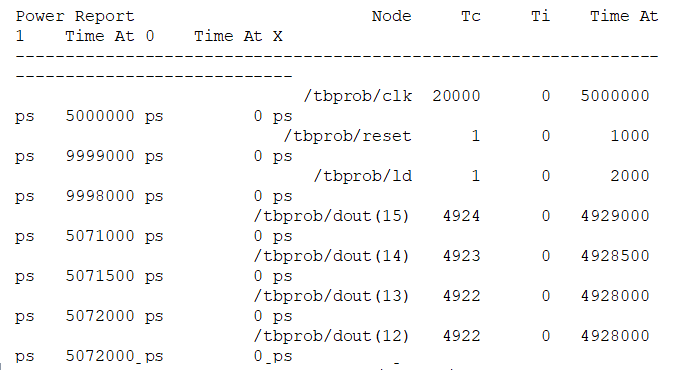
\includegraphics[scale=1]{immagini/fig1_2}
	\caption{\textit{Probabilità e Switching Activity stimati manualmente}}
	\label{fig1_2}
\end{figure} \\
Si riportano nella tabella \ref{tab1}, i risultati ottenuti dalle varie simulazioni.
\begin{table}[!h]\footnotesize
	\centering
	\begin{tabular}{|c|c|c|c|c|}
		\hline
		\textbf{Tc(CK)} & \textbf{Tc(INV)}& \textbf{Tc(AND)}& \textbf{Tc(OR)} &\textbf{Tc(XOR)}\\
		\hline
		20 & 1  & ?& 4&4\\
		\hline
		200 &  43 &40&42& 44\\
		\hline
		2000& 533& 418&352&470\\
		\hline
		20000& 4916& 3606&3784&4876\\
		\hline
	\end{tabular}
	\caption{\textit{Risultati simulazione}}
	\label{tab1}
\end{table}\\
Dai seguenti valori è facile ricavare i valori di Switching Activity simualte, in quanto si possono stimare da:
\begin{center}
	$ A=\frac{Tc(PORT)}{T_{CLK}} $
\end{center}
Come ci si aspettava, essendo la Switching Activity il numero di toogle avvenuti in un periodo, i valori delle simulazioni vengono molto simili ai valori calcolati analiticamente. Aumentando il tempo di simulazione, i valori di Switching Activity diventano sempre più precisi, arrivando ad avere un errore tra 0,01-0,5.

\section{Probability and Activity Calculation: Simple Logic Gates}